% %%%%%%%%%%%%%%%%%%%%%%%%%%%%%%%%%%%%%%%%%%%%%%%%%%%%%%%%%%%%%%%%%%%%%%%%%%%%%
% %%%%%%%%%%%%%%%%%%%%%%%%%%%%%%%%%%%%%%%%%%%%%% Introduction to Pc4 Pulsations
% %%%%%%%%%%%%%%%%%%%%%%%%%%%%%%%%%%%%%%%%%%%%%%%%%%%%%%%%%%%%%%%%%%%%%%%%%%%%%

\chapter{Magnetic Pulsations}
  \label{ch_pc4s}



\begin{longtable}{ @{\extracolsep{\fill}} cccccccc @{\extracolsep{\fill}} }
  \caption[IAGA Magnetic Pulsation Frequency Bands]{IAGA Magnetic Pulsation Frequency Bands\cite{jacobs_1964}}
  \label{tab_iaga} \\

  \toprule
  &
  Pc1 &
  Pc2 &
  Pc3 &
  Pc4 &
  Pc5 &
  Pi1 &
  Pi2 \\
  \midrule
  \endfirsthead

  % Footer for the end of the table
  \bottomrule
  \endlastfoot

  Period (\si{\second}) &
  1--5 &
  5--10 &
  10--45 &
  45--150 &
  150--1000 &
  1--20 &
  20--1000 \\

  Frequency (\si{\mHz})&
  200--1000 &
  100--200 &
  22--100 &
  7--22 &
  1--7 &
  25--1000 &
  1--25 \\

\end{longtable}



\todo{A few sentences about Pi1 pulsations. Frequency range, when/where they are seen, and why they are interesting. }

\todo{Pi2. }

\todo{Pc1. }

\todo{Pc2. }

\todo{Pc3. }

\todo{Pc4. }

\todo{Pc5. }

\section{Field Line Resonance}

It seems like we should probably have a section called ``Pc4 Pulsations''... but won't we mostly be talking about the idea of FLRs?

\section{Giant Pulsations}


%
% From W J Hughes' Magnetospheric ULF Waves: A Tutorial With a Historical Perspective
%

% rolf 1920 for early observation of Pi2
% angenheister 1931 for early giant pulsation
% Dungey 1954, 1963 for geomagnetic pulsations along field lines. 

% Jacobs et al 1964 has Pi and Pc classifications
% Sigura 1961 showed simultaneous observations at north and south foot points
% nagata et al 1963 showed that they were standing waves

% Patel 1965 made observations in space, and matched them to observations on the ground
% Cummings et al 1969 numerically integrated Dungey's equations to estimate eigenfrequencies
% soviets discovered that different pulsations have different sources in the 1970s; see troitskaya 1993 and greenstadt and russell 1993
% troitskaya 1969 showed that Pc3 can sometimes be explained by a sudden change in the size of the magnetosphere following an impulse. an example -- this must have also been seen earlier. because... 
% Bolshakova and Troitskaya 1968 showed that Pc3 observation depends on IMF N/S. Iff IMF is within about 50 degrees of the earth-sun linem Pc3 is observable on the ground. 
% Troitskaya et al 1971 showed Pc3 frequencies at L=3 depend on IMF magnitude
% Gul'elmi 1974 and Kovner et al gave theoretical justification for these observations. 
% Russell and Hoppe 1981 made observations upstream of the bow shock to unify some ideas. upstream waves are driven by ion cyclotron instability, which depends on IMF magnitude. 

% Gringauz et al 1970 found that solar wind number density affects Pc3 and Pc4 periods (oppositely). The Pc4 effect is a standing question. 

% Samson et al 1971 new observations with digital recording and arrays near the plasmapause! they showed MLT dependence of peak amplitude, and different regions of opposite circular polarization. 
% Dungey 1954 had suggested KH as a wave energy source, which explained the flipping circular polarization at noon. 
% Southwood 1974 went back to the equations and came up with a reason for resonance. waves hitting the bow shock propagate in as an evanescent fast mode. when it gets to a resonant field line, the fast mode couples to the shear mode. the energy tunnels. this only happens if dissipation is finite. 
% Chen and Hasegawa 1974 did too, independently
% Newton et al 1978 showed that joule dissipation at the ionosphere is dominant, and that the amount of dissipation determines the width of the resonance. 

% kivelson et al 1984 argued for cavity mode eigenfrequencies. Pc5. 
% kivelson and southwood 1985, 1986 did analytical work to defend it. 
% Lee and Lysak 1991 did numerical work in a dipole geometry. 

% Harrold and Samson 1992 The waves probably have to be reflected by the bow shock, not by the magnetopause, to line up with the observed eigenfrequencies. 1 to 3 mHz. 

``To summarize, the general buffetting of the magnetosphere by variations in the solar wind dynamic pressure, or perhaps by sporadic magnetic reconnection, provides a broad band energy source to the magnetosphere. The magnetospheric cavity as a whole rings at its own eigenfrequencies, thus transporting energy at just those frequencies to field lines deep in the magnetosphere. Those field lines whose eigenfrequencies match one of the cavity eigenfrequencies couple to the cavity mode and resonate strongly, producing the classical field line resonance signature.\cite{hughes_1994}'' 

% allan et al 1985 did early observation of ULF waves (Pc5 and Pc4) from waveform plots. 
% Waters et al 1991 ground-based observation of Pc3 and Pc4 before spacecraft existed at small L. 
% Menk et al 1993 also

Dungey's \Alfven wave paper\cite{dungey_1954}. 

High-modenumber ULF pulsations are damped by the ionosphere, making it more difficult to observe them on the ground\cite{hughes_1976}. Small structures are also damped; resonances narrower than $\sim \SI{100}{km}$ aren't visible on the ground. 

\todo{See also Glassmeier and Stellmacher, 2000 (about small latitude), and Wright and Yeoman, 1999, Yeoman and Wright, 2001 about large \azm}

Multi-spacecraft observation of a ULF wave with very high modenumber (70+) and no apparent ground signature\cite{takahashi_2013}. 

A recent survey of Van Allen Probe data showed that Pc4 pulsations -- the poloidal ones, at least -- occur primarily during geomagnetically active times, near the plasmapause, over just a handful of hours of dayside MLT\cite{dai_2015}. This confirmed and refined older work\cite{engebretson_1987}. 

ULF waves have been shown to correlate with pulsating aurora and with chorus\cite{jaynes_2015}. It's believed that (in the case presented) substorm injection drove Pc4-5 pulsations, which modulated chorus waves, which pitch-angle scattered electrons with energies on the order of \SI{10}{\kilo\eV}. 

Energetic ring current and radiation belt particles can be accelerated by ULF waves through drift or drift-bounce resonance\cite{southwood_1976}. 

A Hall-conducting ionosphere reflects ULF waves\cite{hughes_1974}. 

``It is not clear why noncompressional [high-\azm] Pc4 poloidal waves, which are presumably driven by instability within the magnetosphere, preferrentially occur on the dayside.\cite{dai_2015}''

Poloidal and toroidal ULF polarizations are treated differently by the ionosphere\cite{greifinger_1968} (or, more recently, \cite{fujita_1988}).  

\todo{Theoretical consideration of decay vs propagation, by frequency. Lysak and Yoshikawa 2006. }

\todo{Fishbone instability. McGuire 1983, Chen 1984. Similar phenomenon, but for lab plasmas. }

An ideal poloidal mode decays to the toroidal mode in the presence of curved magnetic field lines\cite{radoski_1974} or a gradient in the \Alfven speed\cite{mann_1995}. The time is proportional to the azimuthal wavenumber\cite{mann_1995}. An analytical follow-up agreed with the numerical work\cite{mann_1997}. 

\todo{Mann gives the poloidal-to-toroidal decay time to be $\tau = \frac{d \lambda}{d \omega_A'}$, where $\lambda = \frac{\azm}{2 \pi r}$ and $\omega_A'$ is the spatial derivative of the \Alfven bounce frequency, but this doesn't seem to line up. When $\tau$ is computed using our \Alfven bounce frequencies, the result is much less than \SI{1}{\second}. Double-checking is necessary. }

Analysis of GOES data from 2008 to 2013 shows about 100 Pg events. They are concentrated on the morningside. No particular correlation with storm phase\cite{motoba_2015}. 

Recall compressional poloidal Pc4s are mostly during storm time, and noncompressional are mostly specifically during late recovery\cite{dai_2015}. Only 19 fundamental poloidal mode examples were identified from the 390 noncompressional poloidal events. 

Pgs are rare\cite{brekke_1987}. 

Most Pgs observed on the ground have \azm in the range 16 to 35\cite{takahashi_1992}. 

Poloidal Pc4s may be caused by phase space gradients\cite{dai_2013}. 

Fundamental standing waves are possibly excited by drift resonance of ions with energy around \SI{100}{\kilo\eV}\cite{thompson_2001,dai_2013}. 

``It is unclear whether other generation mechanisms of fundamental standing waves such as drift wave instability\cite{green_1979} can explain the localization of Pgs in local time (LT).''\cite{motoba_2015}

Motoba\cite{motoba_2015} found \azm valuse in the range 10 to 15 for a sample of Pgs. Previous studies\cite{rostoker_1979,glassmeier_1980,hillebrand_1982,poulter_1983} are in general agreement that Pg modenumbers fall into the range 16 to 35. 

Another past study: \cite{takahashi_1984}. Satellite data is surveyed and classified by polarization, harmonic, wavenumber, etc, in order to determine the mechanisms for generating \Alfven waves. Old, but still pretty representative, according to Motoba\cite{motoba_2015}. 

It seems to be the convention to find a Pg event on the ground, then look at satellite data. That's certainly what was done in \cite{motoba_2015}. 

Per \cite{motoba_2015}, most Pg events happen around $L=7$, but some do happen near the plasmapause, as seen(?) by \cite{green_1985}. 

``The AL distribution shown in Figure 14c are consistent with the findings of \cite{rostoker_1979} that Pgs occur as the magnetosphererecovers from previous activities (substorms).''\cite{motoba_2015} Finds this to be reasonable because it's ``very likely'' that energetic ions injected into the inner magnetosphere from the magnetotail provide energy to Pgs. 

Second harmonic poloidal waves -- as most of \cite{dai_2015}'s events are -- are unlikely to cause a Pg event on the ground\cite{takahashi_1992}. 

\cite{cummings_1969}: Standing \Alfven waves in the magnetosphere. Theoretical fundamental toroidal and poloidal modes can vary by up to \SI{30}{\percent} in frequency. 

\cite{motoba_2015} suggests that Pgs originate from the fundamental poloidal mode waves at all local times. 

First Pg observation\cite{birkeland_1901}. 

Energetic particles can get accelerated (or deaccelerated) by the wave electric field through the drift or drift-bounce resonance\cite{elkington_1999}. 

Poloidal ULF waves are capable of energizing radiation belt electrons (not ions?)  to very high energy through coherent drift/drift-bounce resonance interactions\cite{elkington_1999,ozeke_2008,mann_2013}. By multiple wave-particle interactions, poloidal ULF waves can lead to radial diffusion of radiation belt particles\cite{elkington_2003,tu_2012,ozeke_2012}. 

AMPTE/CCE data has shown a correlation between poloidal Pc4 activity and intense ring current flux near the equator\cite{engebretson_1988}. 

Pc4 pulsations are radially localized, per multiple satellite observations\cite{engebretson_1992}, and spread no more than about 8 hours MLT. They peak around $L$ of 5 to 6, with lower occurrence rate 2.5 to 9\cite{anderson_1990,liu_2009}.

Low \azm is compressional\cite{hughes_1994}. Drivers may include KH at the magnetopause\cite{chen_1974,southwood_1974,liu_2011}, variations in solar wind pressure (such as interplanetary shocks)\cite{zong_2007,zong_2009,hao_2014,degeling_2014,kessel_2008}, and waves in the foreshock region\cite{russell_1983,takahashi_2015}. 

At high \azm, the poloidal mode decouples from the compressional mode\cite{hughes_1994} and becomes guided\cite{cummings_1969}. 

Most observed guided waves are second harmonic excited by the drift-bounce resonance\cite{hughes_1978,singer_1982,takahashi_1990}. Fundamental modes, driven by drift resonance, are rarer, but have been observed\cite{dai_2013}. 

The plasmapause -- representing a sharp change in \Alfven speed -- is important for ULF waves. Waves are trapped and scattered by the effective potential well, analogous to \Schrodinger's equation\cite{lee_1998,lee_1999,dai_2009}. This has been shown theoretically\cite{klimushkin_1998,leonovich_2000,klimushkin_2004,mager_2013} (most recent is \cite{mager_2013}) and observationally\cite{takahashi_2009,takahashi_2010}. 

Because the inner magnetosphere is low-$\beta$ (that is, magnetic pressure dominates thermal pressure), the strength of the compressional-poloidal coupling indicates \azm\cite{hughes_1994}. 

\todo{How so? }

\todo{Haven't read this paper yet, but it looks fun: \cite{glassmeier_2004}. }

Pc5 waves peak around $L$ of 7 to 9, too far out for RBSP\cite{anderson_1990,liu_2009}. 

It's perhaps not surprising that, finding events based on ground signatures, \azm would skew low. High-\azm waves can't penetrate the ionosphere. 

Compressional waves come from the outer boundary, propagating across field lines\cite{lysak_1992}. 

Compressional driving doesn't preclude drift or drift-bounce resonance\cite{zong_2007,zong_2009}. 

Plasmapause refilling may cause onset of the instability that drives noncompressional Pc4s\cite{engebretson_1992,liu_2013}. 

Note that Dai\cite{dai_2015} was pretty generous about what counted as a storm... anything that hits \SI{-30}{\nano\tesla}. So \cite{motoba_2015} may not have counted the same way when they found no particular correlation with storm phase. 

Compressional poloidal Pc4 pulsations are much more common during storms, but not particularly sensitive to storm phase. Noncompressional ones occur primarily during recovery\cite{dai_2015,rostoker_1979,engebretson_1992,anderson_1994}. 

In the example shown of a fundamental mode poloidal Pc4, and in the example of a higher harmonic Pc4, a mishmash of toroidal activity is present. \cite{dai_2015}, figure 8 and 9 respectively. 

Poloidal Pc4 pulsations are common inside and outside the plasmapause. Plasmapause peaks at 4.8--5 RE and 5.8--6RE\cite{dai_2015}. 

Drift resonance is the fundamental mode. Drift-bounce is higher harmonics\cite{dai_2015}. 

\todo{Do the unambiguous Pc4 events in \cite{takahashi_2011} and \cite{dai_2013} also have a mishmash of toroidal activity? }

Second harmonic: Br leads Ea by 90 degrees. Fundamental mode: Br lags Ea by 90 degrees. \cite{dai_2015}

Low-\azm waves tend to be more muddled... driven by broadband sources rather than resonance\cite{dai_2015}. 

Fundamental mode is rare. Of 390 noncompressional events, Dai identified 19 to be clearly fundamental mode and 197 to be clearly second harmonic\cite{dai_2015}. 

\todo{Fishbone instability? }

\todo{Lab \Alfven waves as LASP? }

Fast and shear (toroidal and poloidal) modes are coupled by nonzero Hall conductivity\cite{kato_1956}. 

Shear mode incident on the ionosphere, pederson current closes FAC, Hall current then generates a fast mode wave which may be detected in space or on the ground\cite{tamao_1965}. 

Toroidal mode is usually associated with external driving\cite{chen_1974,southwood_1974}. 

Guided poloidal wave arises as \azm goes to infinity\cite{radoski_1967_poloidal}. 

Observations show that the poloidal mode is most excited in the second harmonic\cite{cummings_1969,hughes_1978,arthur_1981,singer_1982,takahashi_1984,engebretson_1988} even when there is a strong compressional component\cite{takahashi_1987,haerendel_1999,vaivads_2001,sibeck_2012}. 

Theoretical justifications for why the second harmonic would be preferrentially excited in the ring current environment\cite{southwood_1976,chen_1991,cheng_1994,chan_1994}. 

The energy of the resonant particle gives \azm, recall $\omega - \azm \omega_d = 0$ or something\cite{ozeke_2001}. 

Giant pulsations happen at large \azm, and do not produce ground signatures\cite{takahashi_2013}. 

Observations of odd-mode poloidal waves... possible fundamental\cite{yang_2010,eriksson_2005}.

Observations in space indicate that Pgs are fundamental poloidal mode\cite{kokubun_1980,hillebrand_1982,kokubun_1989,takahashi_1992,glassmeier_1999}. 

\Alfven waves with small latitudinal scale\cite{glassmeier_2000} or high \azm\cite{wright_1999,yeoman_2001} are screened by the ionosphere. Attenuation factor from \cite{hughes_1976} and \cite{glassmeier_1984} DID NOT PRINT PROPERLY. LOOK IT UP. 

Typical magnitude is order of a few nT, and a few mV/m\cite{takahashi_2013}. 

Drift-wave instability\cite{hasegawa_1971,green_1979,green_1985} is also a possibility for exciting fundamental poloidal waves, though it requires cold plasma, so it could only happen in the plasmasphere. 

Fundamental poloidal mode is drift resonance, not drift bounce\cite{poulter_1983}. 

Pgs are most common during solar minimum, perhaps because of decreased mass loading of heavy ions\cite{denton_2011}. 



The \Alfven speed is computed from Kelley's low-density profile, modified to take into account the local density. The density, in turn, is the sum of a plasmaspheric profile and a high-latitude auroral profile. 
\begin{align}
  \ep &= \text{(low-density tabulated value)} + \frac{ n \bar{m} }{B_0^2}
\end{align}

\todo{What's a clean way of showing the low-density \ep that we read in? }

\todo{Does Kelley list the electric constant or the \Alfven speed? }

Where $\bar{m}$ is the ambient mean molecular mass and $B_0$ is the zeroth-order magnetic field strength, $B_0 = \SI{3.11e4}{\nano\tesla} \lr{ \frac{R_E}{r} }^3 \sqrt{ 1 + 3 \cos^2 \theta }$. Note that \SI{3.11e4}{\nano\tesla} is the value of the Earth's magnetic field at the equator on Earth's surface. 

\todo{Cite this number? Jesse just says it's a ``representative'' number. He uses \SI{30}{\micro\tesla}. }

\begin{figure}[H]
    \centering
    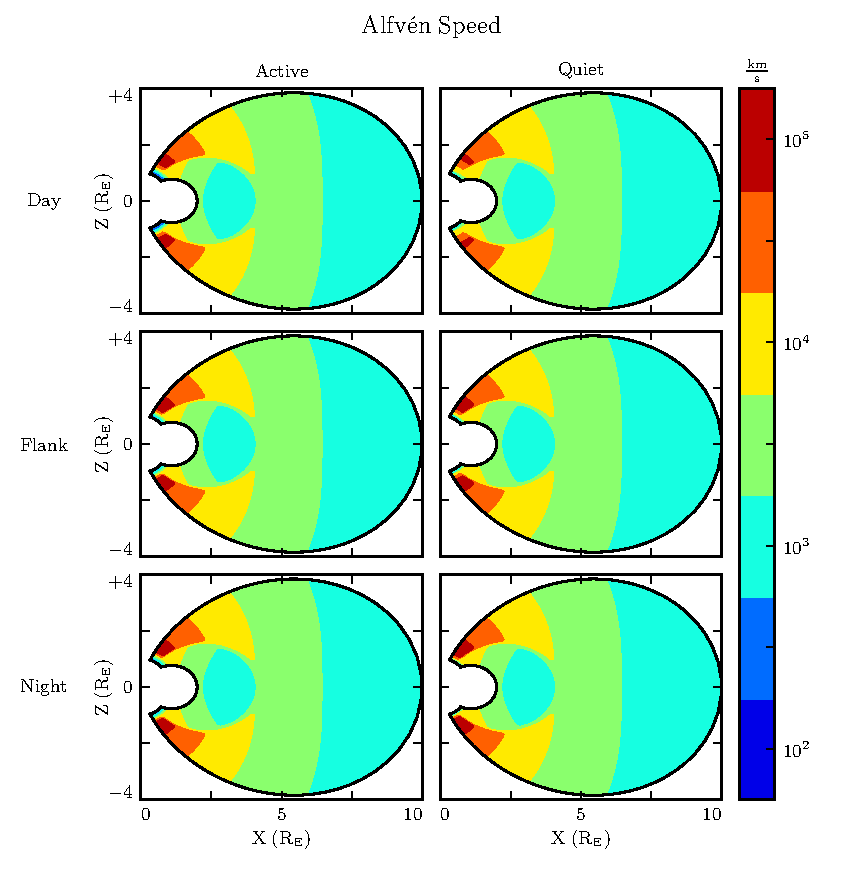
\includegraphics[width=\textwidth]{figures/va.pdf}
    \caption[\Alfven Speed Profiles]{
      \Alfven speed profiles, adapted by Lysak\cite{lysak_2013} from Appendix B of Kelley's textbook\cite{kelley_1989}. 
    }
    \label{fig_va}
\end{figure}

\todo{Above the profile, Bob scales the value that's read in as $r^5$ or something. Is there a citation for that? }

The \Alfven speed is then computed per $\va^2 \equiv \frac{1}{\mz \ep}$. 

\begin{figure}[H]
    \centering
    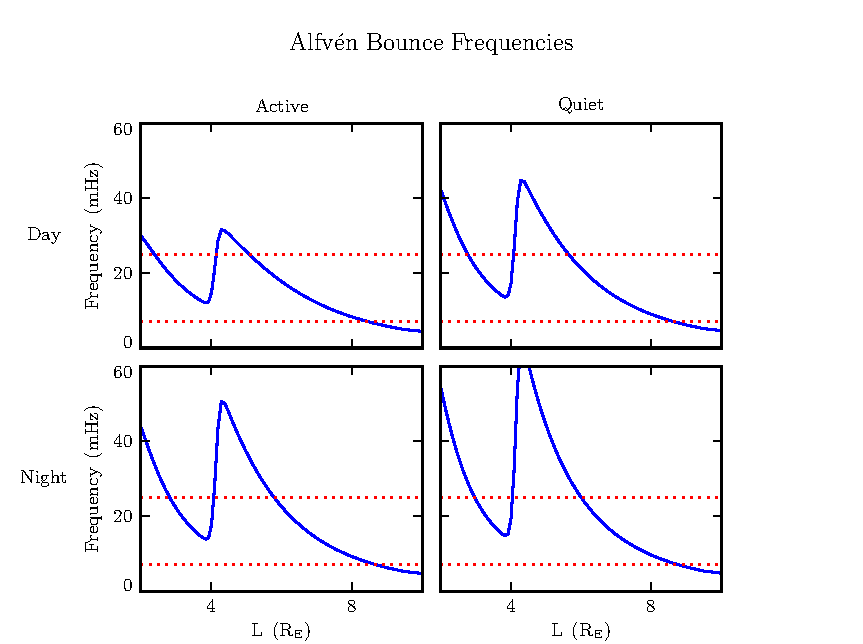
\includegraphics[width=\textwidth]{figures/fa.pdf}
    \caption[\Alfven Bounce Frequency Profiles]{
      \Alfven bounce frequency profiles, computed by integrating the the \Alfven speed back and forth over a field line. $f_A = \lrb{ \oint \frac{dz}{v_A} }^{-1}$. Dotted lines indicate the Pc4 frequency range, \SIrange{7}{25}{\mHz}. In each profile, the effect of the plasmapause is clearly visible, centered at $L=4$. Field lines just inside and just outside the plasmapause appear susceptible to resonance in the Pc4 band. 
    }
    \label{fig_fa}
\end{figure}

\todo{Talk about how the size of the plasmasphere can be adjusted, and \SI{4}{\RE} is just a typical value. }

\todo{Explain how the \Alfven speed constrains the time step. }



